% Copy to docs/ambiguities/lectureNN/main.tex when actual questions arise.
% Replace NN and the title; add real LNN-Qxx entries from the lecture ledger.
% Build from the repository root: make questions LECTURE=NN
% Store evidence crops in the new project's images/ folder.
% Questions are for later review. Do not stop transcription or ask live chat
% questions; deliver this PDF with the lecture, keeping unresolved items marked.
\documentclass[a4paper,12pt]{article}
\usepackage[margin=19mm]{geometry}
\usepackage{amsmath,amssymb,graphicx,xcolor}
\usepackage{fontspec}
\usepackage{xepersian}
\settextfont{XB Roya}
\setlatintextfont{Latin Modern Roman}
\definecolor{ink}{HTML}{173D75}
\graphicspath{{images/}}
\setlength{\parindent}{0pt}
\setlength{\parskip}{5pt}
\linespread{1.12}
\newcommand{\qtitle}[2]{{\Large\bfseries\color{ink} پرسش \lr{#1}: #2}\par}
\newcommand{\answer}{\medskip\textbf{پاسخ یا صورت مورد تأیید و تاریخ:}\par\vspace{18mm}\hrule\medskip}
\begin{document}
{\LARGE\bfseries پرسش‌های ابهام جلسهٔ \lr{19}}\par
{\large جزوهٔ جبر پیشرفتهٔ دکتر خسروی}\par
شمارهٔ صفحه‌ها، شمارهٔ یک‌مبنای صفحه در فایل پی‌دی‌اف است، نه شمارهٔ دست‌نویس.
پرسش‌های حل‌نشده هنوز در اسلایدها به‌عنوان متن قطعی پذیرفته نشده‌اند.
\medskip\hrule\medskip

\qtitle{L19-Q01}{ترتیب عوامل در آغاز اثبات حفظ شکافتگی}
\textbf{وضعیت:} باز؛ خوانش موقت، بدون پاسخ کاربر. ثبت در ۲۰۲۶/۱۰/۲۵.\par
\textbf{نشانی منبع:} نسخهٔ یگانهٔ \lr{primary}، صفحهٔ ۱۲، یک‌سوم بالای صفحه؛
آغاز اثبات قضیهٔ انتهای صفحهٔ ۱۱.\par
\begin{LTR}\small\texttt{sources/lectures/19 Tensor product .pdf}\end{LTR}
\textbf{عبارت منبع:} در جملهٔ آغازین «ابتدا $1\otimes f$، یک‌به‌یک بودن را
بررسی می‌کنیم» خوانده می‌شود، در حالی که محاسبهٔ همان بند چنین است:
\[
(h\otimes1)(f\otimes1)=(hf)\otimes1=1\otimes1=\operatorname{id}.
\]
\begin{center}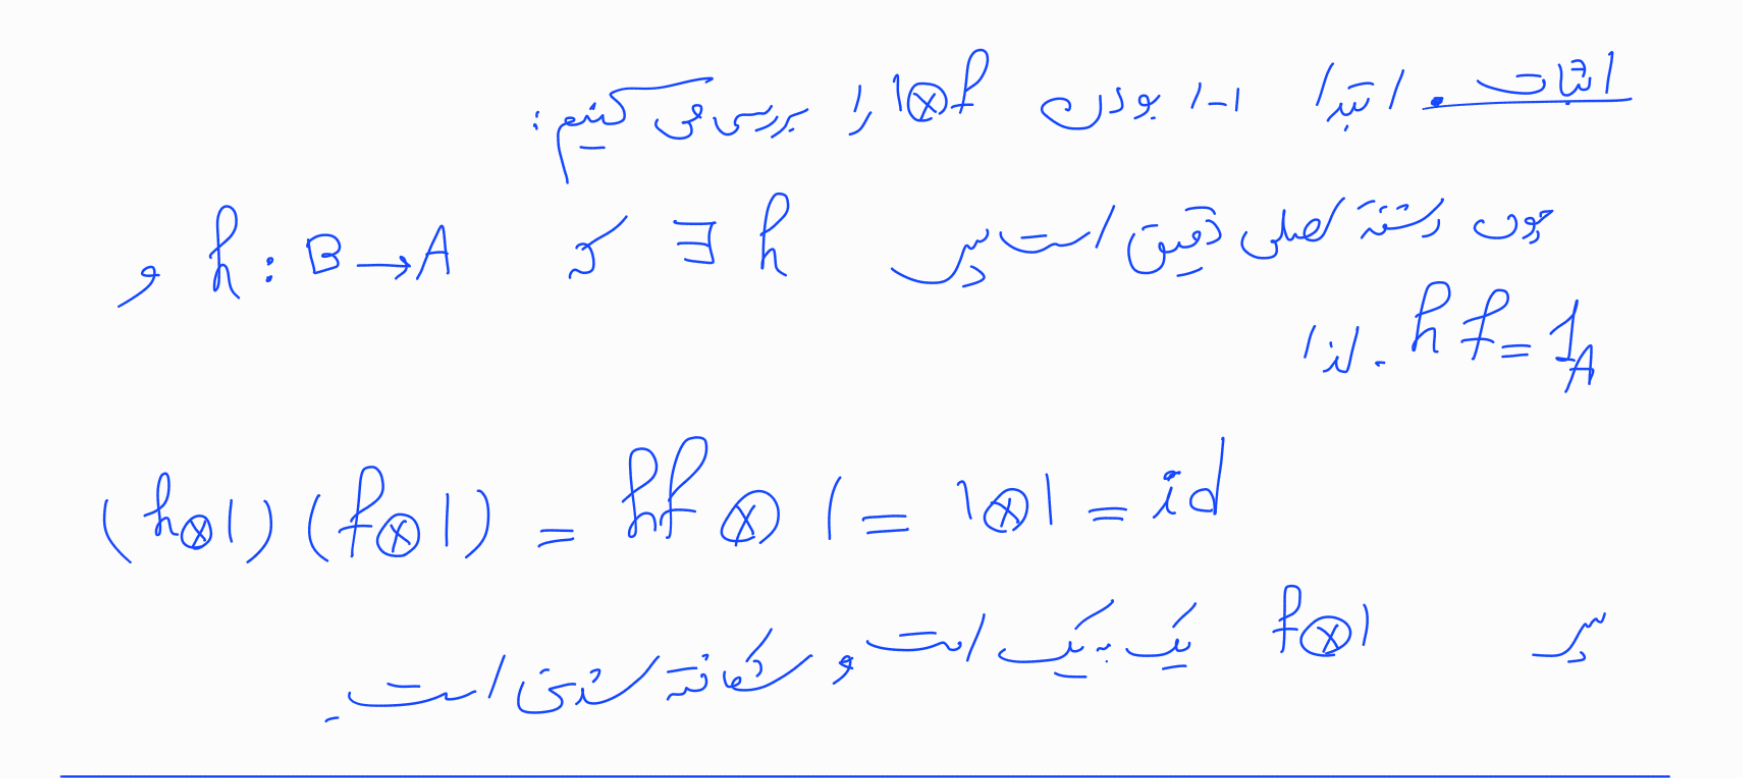
\includegraphics[width=.97\linewidth]{L19-Q01-page12.png}\end{center}
\textbf{خوانش‌های ممکن:} (۱) جملهٔ آغازین باید $f\otimes1$ باشد؛ این خوانش با
دنبالهٔ $A\otimes_R D\to B\otimes_R D$ در قضیه و با محاسبهٔ بالا سازگار است.
(۲) اگر $1\otimes f$ عمدی باشد، باید ترتیب عوامل تانسوری و نگاشت بازپس‌گیری
در این بند نیز متناسب با آن عوض شود؛ چنین تغییری در محاسبهٔ منبع دیده نمی‌شود.\par
\textbf{اثر تفاوت:} دامنه و هم‌دامنهٔ $f\otimes1$ برابر
$A\otimes_R D$ و $B\otimes_R D$ است؛ $1\otimes f$ به ترتیب دیگر عوامل مربوط
می‌شود. این دو نماد بدون تعیین طرف مدول‌ها قابل جایگزینی نیستند.\par
\textbf{پرسش برای بازبینی بعدی:} آیا نماد درست در جملهٔ اول این اثبات
$f\otimes1$ است و $1\otimes f$ خطای نوشتاری است؟\par
\textbf{تصمیم موقت در اسلاید:} محاسبهٔ خود منبع با $f\otimes1$ حفظ شده و
ناسازگاریِ جملهٔ آغازین به‌طور آشکار در اسلاید
\lr{lec19:split-exactness-proof} برچسب خورده است. این تصمیم، پاسخ تأییدشده نیست.
\answer
\end{document}
